\section{Trading-Engine}
\label{chap:te}

For backtesting and live execution of trading strategies, a Java framework was built.
This chapter describes the use cases as well as the most important components of the trading engine.

\subsection{Use Cases of the Trading-Engine}
\label{chap:te-use-cases}

The developed trading engine represents a flexible and modular software platform that covers various use cases in the field of algorithmic trading.
The focus is on combining usability, adaptability, and performance.
The following are the most important use cases and features:

\begin{enumerate}
    \item \textbf{Backtesting trading strategies:} The trading engine enables the simulated execution of trading strategies on historical market data.
    This allows strategies to be tested under realistic conditions and their performance, robustness, and risk characteristics to be evaluated.
    By replicating historical market conditions, incorrect decisions can be identified early, and the trading strategy can be adjusted without using real capital.
    \item \textbf{Live execution in real-rime operation:} In addition to backtesting, the engine also supports real-time execution of strategies in the market.
    Through an interface to brokers, the engine can receive market data in real time, make trading decisions, and execute orders directly.
    This enables the engine to be used as the basis for automated trading in production environments.
    \item \textbf{Using money and risk management strategies:} An important use case is the implementation of different money and risk management approaches.
    Users can integrate various strategies for position sizing, stop-loss setting, or profit-taking, and examine their impact on strategy performance in backtests or in live operation.
    This supports the development of more stable and profitable trading approaches.
    \item \textbf{Connecting to any broker:} The trading engine is designed to connect to various brokers via interchangeable interfaces.
    This allows the engine to be combined with different trading systems and platforms.
    This flexibility enables its use in a wide variety of markets and infrastructures.
    \item \textbf{Development and integration of custom trading strategies:} A key feature of the engine is the ability for users to implement their own trading strategies.
    A clear separation between core functionality and strategy logic allows for flexible integration and testing of individual algorithms.
\end{enumerate}

\noindent
Most components of the trading engine are interchangeable and can be implemented by the user.
Only the core of the framework, including the fundamental process flow and control logic, remains fixed.
This allows users to tailor the engine to their individual needs, develop their own modules for data feeds, order management, strategy, or risk control, and thus ensure a high degree of flexibility in the use and further development of the platform.

\subsection{Architecture}

The trading engine consists of many modules ,which can be clustered into three main categories:

\begin{enumerate}
    \item Core Modules (Trading Engine)
    \item Applications
    \item Adapters
\end{enumerate}

\noindent
\autoref{fig:te-components} shows the components of the trading engine.

\begin{figure}[H]
    \centering
    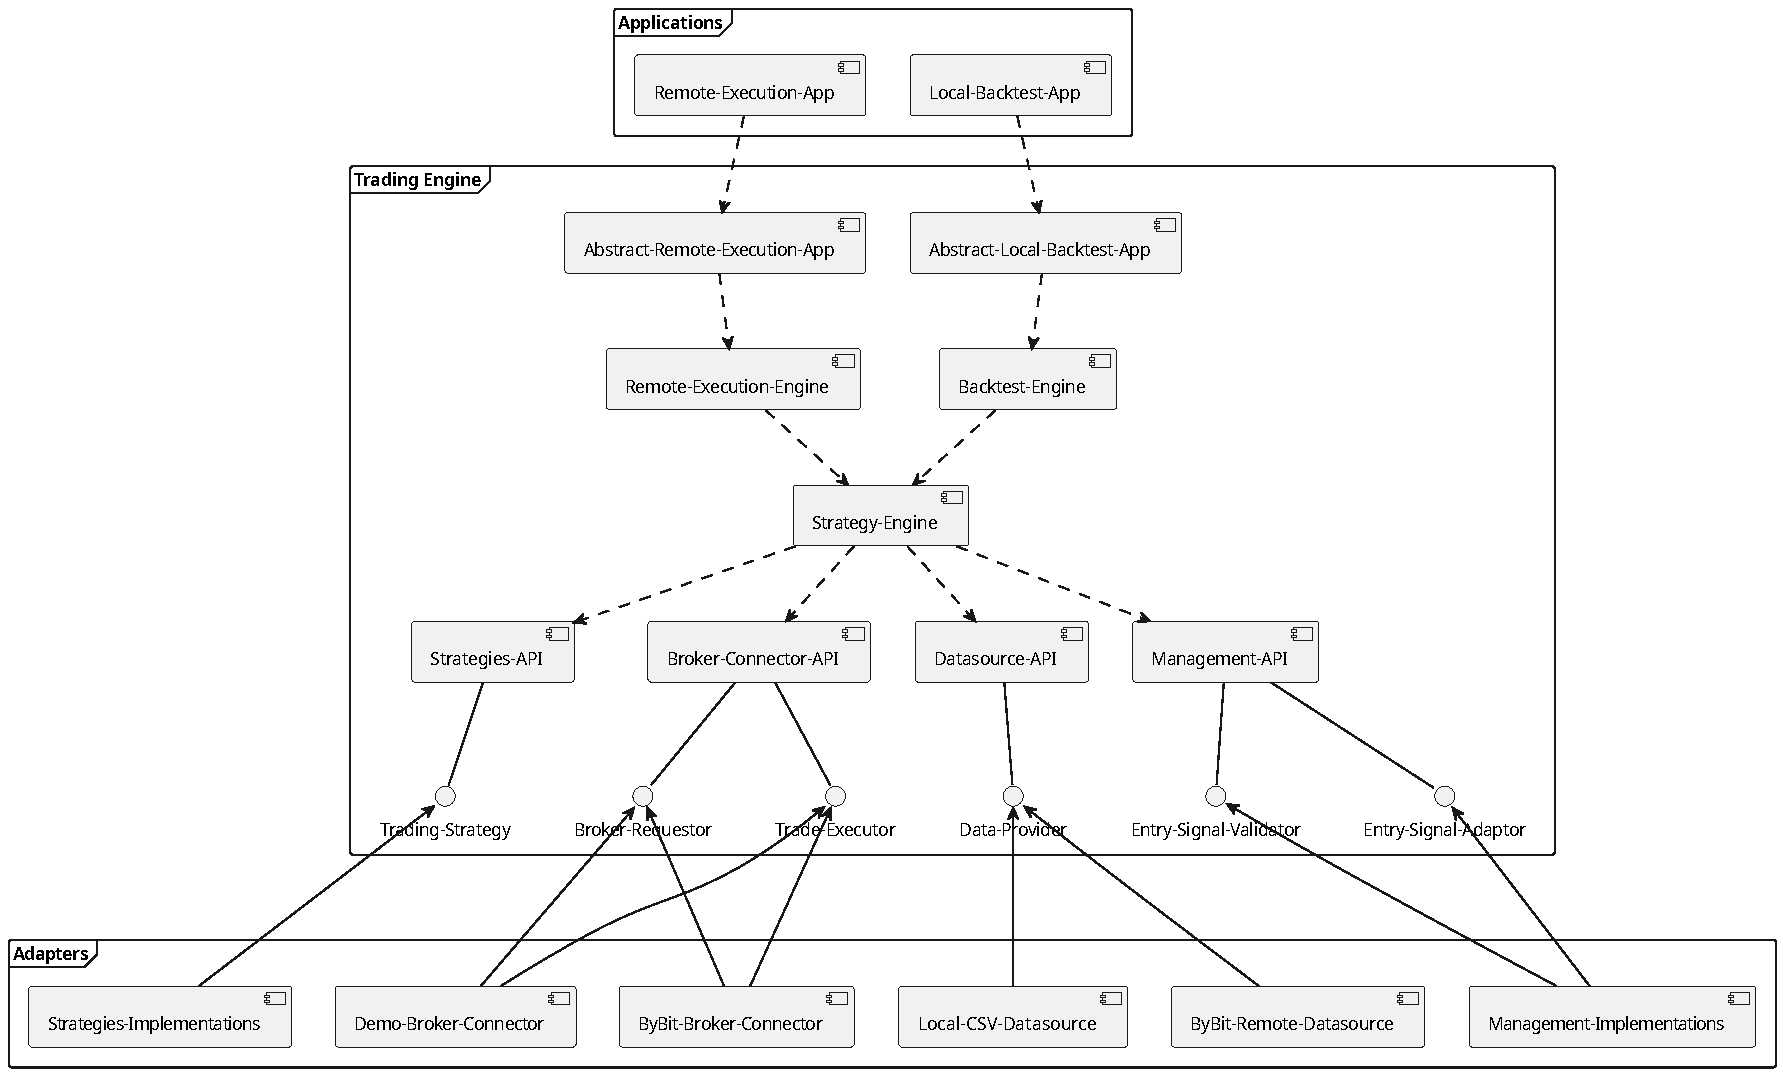
\includegraphics[width=\textwidth]{images/trading-engine/trading-engine-components}
    \caption{Trading Engine Components}
    \label{fig:te-components}
\end{figure}

\subsubsection{Plugin Architecture}

To achieve the flexibility mentioned in \autoref{chap:te-use-cases}, a plugin architecture was used.
Within the core, interfaces have been defined specifying which external functionalities are required (Service Provider Interface, or SPI).
To facilitate seamless interchangeability for users, the implementations of the interfaces in the external modules (Adapters) are loaded by the Java \texttt{java.util.ServiceLoader}.

The \texttt{ServiceLoader} loads classes at runtime that implement a specific interface or abstract class.
The classes to be loaded are specified via a configuration file in the \texttt{resources/}\\\texttt{META-INF/services} directory, which the \texttt{ServiceLoader} searches for in every JAR file in the classpath.
If a corresponding configuration file is found, the \texttt{ServiceLoader} can create an instance of the respective class using the default constructor \cite{java-service-loader}.

As an example, a Service Provider Interface for read access can be defined in a module named \texttt{spi}.

\lstinputlisting[language=Java, caption=SPI Definition, label=lst:service-loader-spi-definition, style=java]{java/trading-engine/service-loader-base.java}

\noindent
This interface can be implemented in multiple modules.
One implementation can be used to read data from files:

\lstinputlisting[language=Java, caption=File Repository Implementation, label=lst:service-loader-file, style=java]{java/trading-engine/service-loader-file.java}

\noindent
Here, a configuration file named \texttt{com.example.spi.read.ReadRepository} is located in the directory \texttt{resources/META-INF/services}.
This file contains the fully qualified class name of the implementation class (\texttt{com.example.adapter.file.read.}\texttt{FileReadRepository}).

\newpage
Another implementation can be used to read data from databases:

\lstinputlisting[language=Java, caption=Database Repository Implementation, label=lst:service-loader-db, style=java]{java/trading-engine/service-loader-db.java}

\noindent
Similar to the \texttt{FileReadRepository}, a file named \texttt{com.example.spi.read.ReadRepository} is located in the directory \texttt{resources/META-INF/services}.
However, this file contains \texttt{com.example.adapter.database.read.DatabaseReadRepository}.

The \texttt{ServiceLoader} searches in each JAR file in the classpath for files under \\\texttt{resources/META-INF/services} with the name \texttt{com.example.spi.read.}\texttt{ReadRepository} that contains the implementation of this interface, and creates them.

Since an external application has the ability to define the classpath, it can add or remove specific JARs.
This allows it to determine which implementations to use.
For example, it can decide to add only the \texttt{file-adapter} module or, if necessary, the \texttt{db-adapter} module if loading from a file, and a database simultaneously.

\subsubsection{Core Modules}

The core of the framework consists of several loosely coupled components that communicate with each other through well-defined APIs.
The most central unit is the \texttt{Strategy Engine} which contains the main logic for the execution of trading strategies, and controls the cooperation of the other subsystems.

The following components form the core:

\begin{enumerate}
    \item \textbf{Data Provider:} Obtains market data via a configurable \texttt{Datasource API}.
    The specific data source (local or remote) is integrated via adapters.
    \item \textbf{Trading Strategy:} The actual trading logic is integrated via the \texttt{Strategies API}.
    This API is separate from the framework and can be extended as required.
    \item \textbf{Broker Requestor \& Trade Executor:} Both communicate with brokers via a generic \texttt{Broker Connector API}, and enable both order placement and broker status queries, such as the current account balance or all open positions.
    \newpage
    \item \textbf{Entry Signal Adapter \& Entry Signal Validator:} These two components process and validate generated entry signals.
    They are linked to the \texttt{Management API} and enable additional risk checks, such as capital requirements or position limits.
    Currently, the implemented management includes all techniques introduced in \autoref{chap:risk-man} and is executed every time a strategy creates an entry signal.
\end{enumerate}

\noindent
Before the \texttt{Strategy Engine}, there are two other engines, named \texttt{Remote Execution}\\\texttt{Engine}, and \texttt{BacktestEngine}, which configure the \texttt{Strategy Engine}.
The difference between the engines is that the \texttt{Remote Execution Engine} defines the \texttt{Strategy Engine} asynchronously.
This means that a remote data source can stream market data via an API.
When new data arrives, the \texttt{Strategy Engine} is notified by the data source and starts executing the trading strategy.
For a local backtest, the \texttt{Strategy Engine} is configured so that data synchronization is handled by the \texttt{Backtest Engine}, not by the data source.

Abstract apps are modules that accept and parse user configurations.
For example, the task of the \texttt{Abstract Local Backtest App} is to ask the user via the console which strategy should be used for the backtest.
With the \texttt{Abstract Remote Execution App}, the configuration is not done via the console but primarily via environment variables.
The parsed configurations are then passed to the respective engines.

\subsubsection{Applications}

The application layer defines specific execution environments by defining the classpath with adapters.

\begin{enumerate}
    \item \textbf{Local-Backtest-App:} Executes trading strategies offline by using the \texttt{Local CSV }\\\texttt{Datasource} and the \texttt{Demo Broker Connector}.
    \item \textbf{Remote Execution App:} Executes strategies in real time and communicates with live broker interfaces.
\end{enumerate}

\noindent
Each application contains its own \texttt{main} method, which constructs and starts the respective implementation.

\subsection{Demo Broker}

For local backtests, the connection to a real broker must be mocked.
Therefore, the \texttt{Demo Broker Connector} is used to replace a real broker.
It takes over the main tasks including:

\begin{enumerate}
    \item \textbf{Order execution and position management:} Executing market, limit, take-profit, and stop-loss orders, including execution fee calculation.
    \item \textbf{Adapt trailing stop positions:} Monitoring trailing stop positions, and adapt the stop-level according to the most recent price.
    \item \textbf{Account balance management:} Managing the available account balance as well as the margin balance.
    \item \textbf{Store executed trades:} Storing the executed trades is essential for risk management and later analysis.
\end{enumerate}

\subsubsection{Order Execution and Position Management}

In the context of trading, order execution and position management are closely connected, because positions can be translated into three orders, where only two of them are actually executed.
As described in \autoref{chap:dealing-with-trading-fees}, it is necessary that the trading engine supports market and limit orders.
In real-life environments, most orders are not executed at the expected price, due to slippage \cite{ig-slippage}.
To simulate slippage, the trading engine can either use historical data of the underlying cryptocurrency, which is available in the lowest available timeframe (usually seconds or tick data), or simulate slippage randomly.
Two problems exist with simulations using historical data.
The first is that data in the seconds or tick range over a long period of time is difficult for private individuals to obtain.
Furthermore, latency must be simulated, which simulates the processing time and network traffic in live operation.
With random simulations, the problem arises that the backtest results are no longer deterministic.
Thus, a subsequent comparison of different strategies is subject to error.
For these reasons, the slippage factor is not taken into account during order execution.
This means that market orders are always executed at the most current available price, and limit orders are always executed at the specified order level.


\autoref{fig:te-position-opening} shows the process of opening a single position.
The margin in euro is calculated using the following formula \cite{margin-calculation}.


\[
    \text{Margin} = \frac{\text{Position Quantity}}{\text{Leverage} \cdot \text{Euro Conversion}} = \frac{\text{Position Size} \cdot \text{Open Price}}{\text{Leverage} \cdot \text{Euro Conversion}}
\]

\noindent
$\text{Euro Conversion}$ is the current price for converting the current counter currency into euros.
For example, for ETH/USDC the $\text{Euro Conversion}$ is the current price of EUR/USDC:
The conversion is done in euros because for different currency pairs with different counter currencies, the margin would be calculated in the respective counter currency.
For ETH/USDC, the margin is calculated in USDC according to the formula.
However, when trading ETH/BTC, the margin is calculated in BTC.
To obtain a result that is always in the same unit, or in this case, the same currency, the additional conversion is implemented.
It is important to note that it is also possible to implement conversion into any currency.
This way, the margin could also be calculated in BTC, for example.
Since USDC/EUR rates are offered by ByBit, it was easier in this case to compute historical data directly from ByBit and obtain the EUR/USDC rate through a conversion $\text{EUR/USDC} = \frac{1}{\text{USDC/EUR}}$.

\begin{figure}[H]
    \centering
    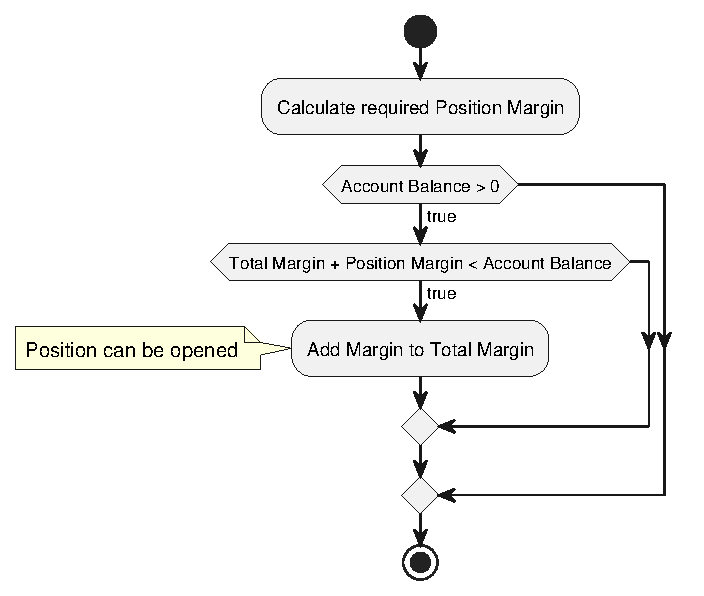
\includegraphics[width=0.7\textwidth]{images/trading-engine/position-opening}
    \caption{Opening a Single Position}
    \label{fig:te-position-opening}
\end{figure}

\noindent
After a position has been opened, it must be closed again at a later point in time.
This can happen either by reaching the stop loss or take profit, or by intentionally closing it, which is controlled by a strategy.
\autoref{fig:te-position-closing} shows the process of closing a single position.
The profit in euro is calculated using the following formula \cite{margin-calculation}:

\[
    \text{Profit} = \frac{(\text{Close Price} - \text{Open Price}) * \text{Position Size}}{\text{Euro Conversion}} *
    \begin{cases}
        -1,& \text{if Sell-Position}\\
        1,              & \text{otherwise}
    \end{cases}
\]

\noindent
Just like with the margin calculation, a conversion into euros also takes place, so that when trading on different pairs with different counter currencies at the same time, the profit is always calculated in the same unit.

\begin{figure}[H]
    \centering
    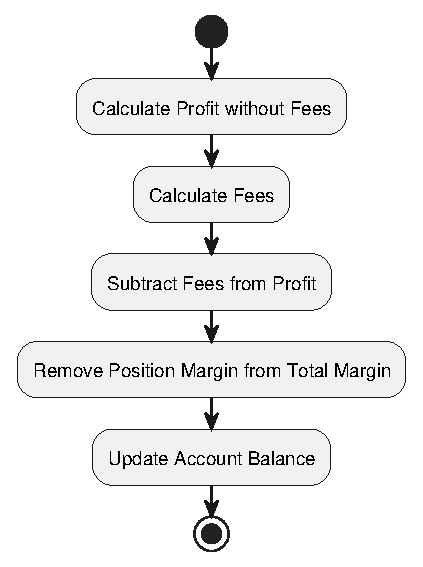
\includegraphics[width=0.4\textwidth]{images/trading-engine/position-closing}
    \caption{Closing a Position}
    \label{fig:te-position-closing}
\end{figure}

\noindent
If there are already positions in a market, the process for opening a new position must be extended.
This is because the size of the open positions must first be reduced, and then a new position (smaller than the original) must be opened.
This is comparable to a netting process.
\autoref{fig:te-complete-position-opening} shows the process of opening a position taking into account that other open positions can already exist.

If a strategy is designed in such a way that all positions in the opposite direction should first be closed when a signal is given in one direction, the strategy must first send an exit signal before the entry signal, which closes all other positions


\begin{figure}[H]
    \centering
    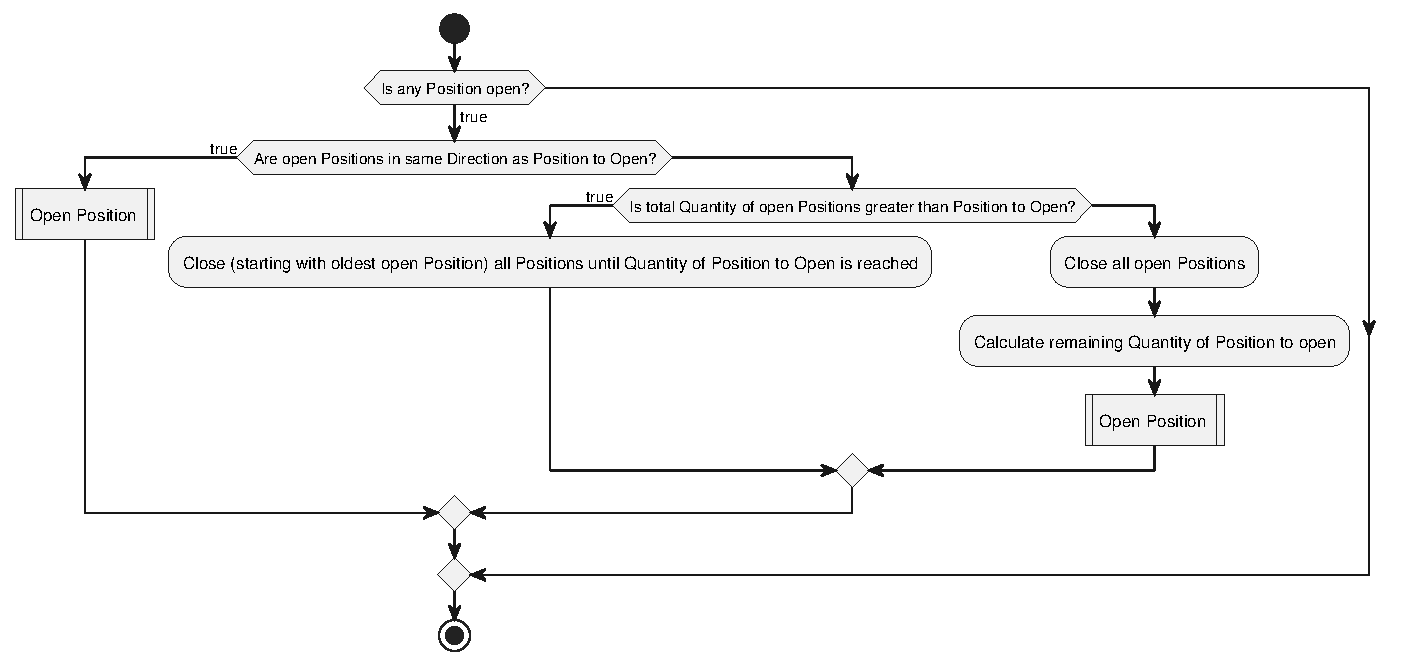
\includegraphics[width=\textwidth]{images/trading-engine/complete-position-opening}
    \caption{Opening a Position}
    \label{fig:te-complete-position-opening}
\end{figure}

\subsubsection{Adapting Trailing Stop Positions}

Trailing stop positions are positions with a dynamic stop order.
The stop level moves automatically with the price as soon as it moves in the desired direction.
For a buy position, the stop level moves if the price rises.
If the price falls, the stop remains unchanged \cite{ig-trailing}.

\autoref{fig:trailing-stop} shows a synthetic closing price (black) and a trailing-stop order with 60 points distance (red) for a buy position.
In the green-filled areas, the price moves in the desired direction, so the trailing-stop level follows the price.
In the red-filled areas, the prices do not move in the desired direction, so the trailing-stop level does not move.
An exception is the red-filled area after $t=3$, where the price moves in the desired direction, but the trailing stop does not.
This is because there is not yet a 60-point gap between the price and the stop level.
Therefore, the stop only moves again once the 60-point gap is restored.

\begin{figure}[H]
    \centering
    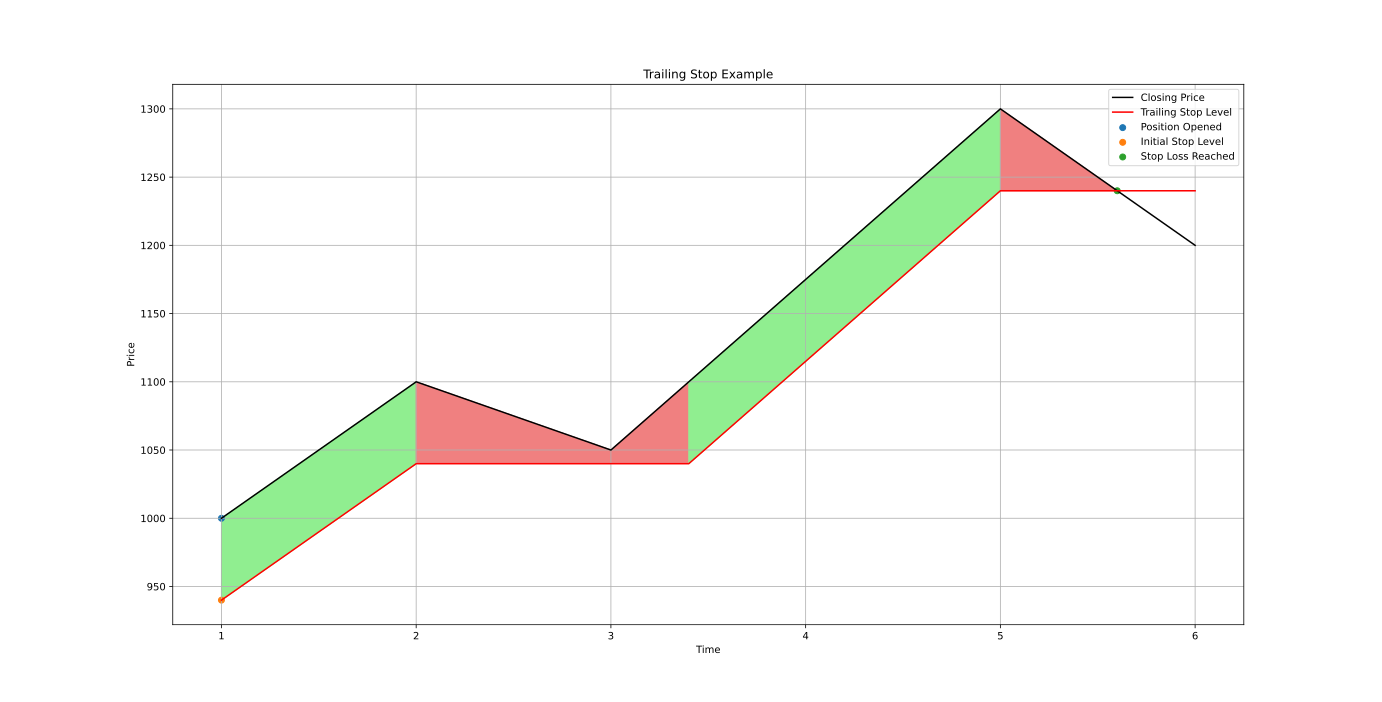
\includegraphics[width=\textwidth]{images/trading-engine/trailing-stop}
    \caption{Trailing Stop Example}
    \label{fig:trailing-stop}
\end{figure}
